\subsection{P2: GPU Model Execution and CPU Confirmation}
P2 使用固定基 Panda/xArm7、匹配键槽与 TCP 有符号 wrench，保留同一
phase prior、反馈 decoder、控制时钟、力限制与成功判据。接触物理和控制
carry 使用 FP64，冻结模型与命令接口使用 FP32。时间 scan 与环境 vmap
形成设备内闭环；IK reset 与工件读写是明确的主机边界。稳态运行通过
禁止隐式设备传输检查；三个条件的完整与 microbatch 结果逐元素一致。

\paragraph{工程语义与物理等价分别验收。}
九个历史开发案例用于工程诊断，其中两个为源身体；它们不是新统计测试集。
27 个保留检查点上，工具侧符号、TCP 力矩平移及 MJX 自身接触集合上的
witness 定义通过独立检查。原 CPU 接触集合与长时闭环等价验收未通过。
% Generated from retained P2 qualification and independent audits.
\begin{center}\small
\begin{tabular}{lrrc}
\toprule
Fixture & CPU & GPU & Long reference \\
\midrule
source\_mode0 & 1 & 1 & Pass\\
source\_mode1 & 1 & 1 & Pass\\
matched\_success & 1 & 8 & Fail\\
matched\_late\_loss & 8 & 1 & Fail\\
matched\_prefix\_force & 9 & 1 & Fail\\
matched\_direct\_loss & 8 & 8 & Fail\\
matched\_direct\_timeout & 5 & 8 & Fail\\
derated\_mode0 & 1 & 1 & Fail\\
derated\_mode1 & 1 & 1 & Fail\\
\bottomrule
\end{tabular}
\end{center}

状态 1/8/9/5 分别表示成功、轴向支撑丢失、力超限和超时。只有两个源
案例满足全部预声明长轨迹容差；有四个案例改变了终止状态。双精度
不能消除接触解算差异及其通过阶段/终止事件累积的影响。
\begin{figure}[ht]\centering
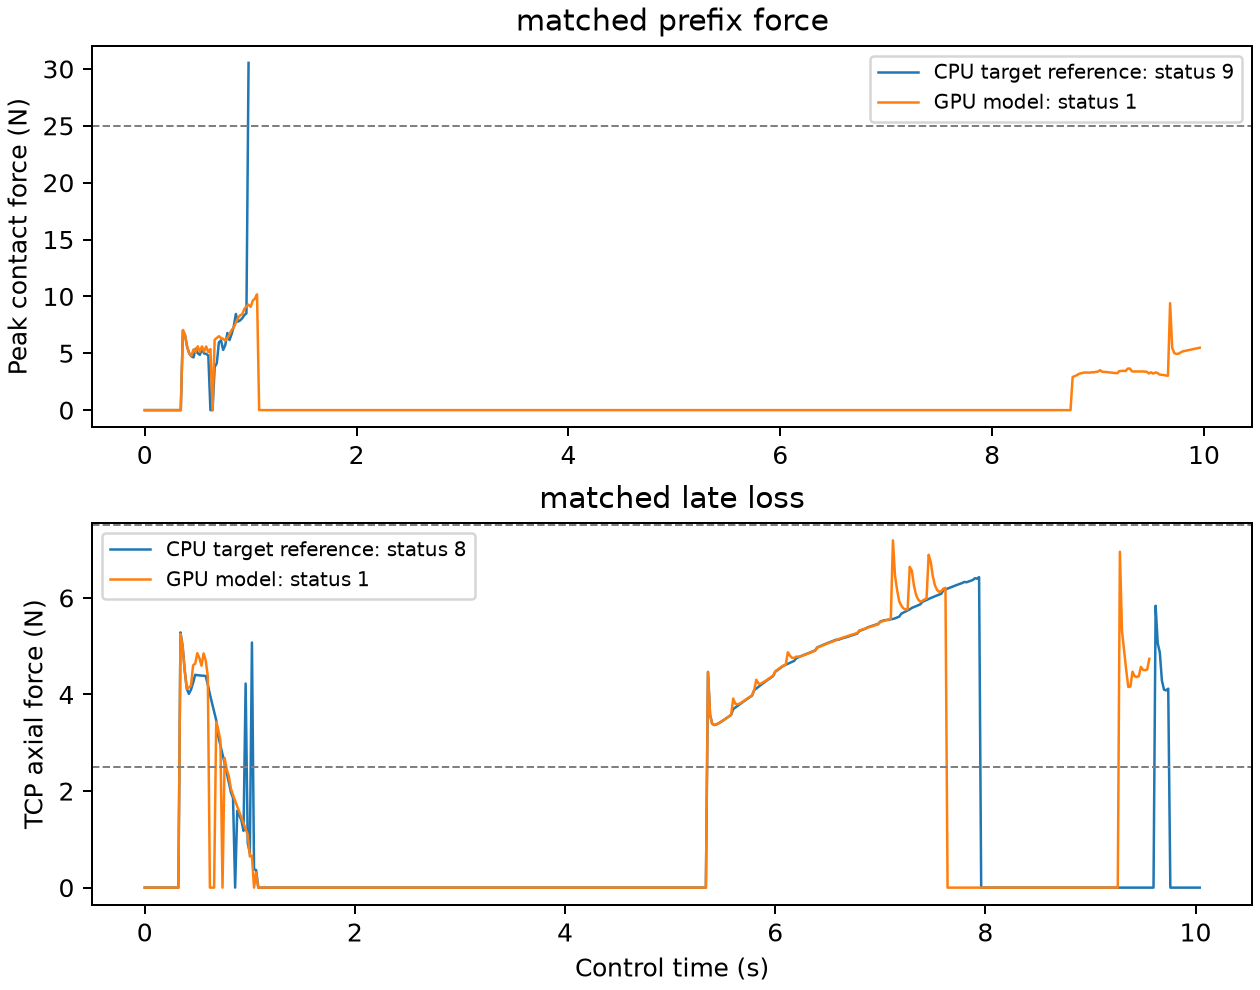
\includegraphics[width=.88\linewidth]{figures/cpu_gpu_contact_discrepancy.png}
\caption{同一冻结 prior/map/reset 的 CPU 与 GPU 接触诊断。上图为峰值
接触力，下图为 TCP 轴向力；虚线为原有约束或保持区间。差异不是方法收益。}
\end{figure}
因此原验收失败保留；另行给予强制独立 CPU 验证的受限模型搜索资格。
GPU 输出不替代 CPU 目标物理，也不自动继承 CPU 校准 twin 的预测准确率。
上述固定诊断中，有界任务成本的最大实测 CPU/GPU 差为 0.80809；
这不是统一误差上界，也不是随机样本总体估计。

\paragraph{扩大覆盖与冻结确认。}
继续引用三份校准重复乘两个条件的已计费 buffer，新增 probe 为零；
没有增加独立校准数。训练 reset 增至 8，独立 CPU 模型验证增至 16，
目标评估与条件 law 各使用 12 个新 reset clusters，均与前轮开发分离。
GPU 搜索完整方法与强 task-only 的同一有限候选池；选中映射经过 CPU
验证后冻结，拒绝仍计入全部请求，最终目标评估使用原 CPU 环境。

共同映射的完整方法为 $46/144$，
强 task-only 为 $70/144$；
\begin{center}\small
\begin{tabular}{lrrr}
\toprule
Method & Derated & Matched & Rejected \\
\midrule
direct & 0/72 & 1/72 & 0\\
full & 22/72 & 24/72 & 96\\
task\_only & 22/72 & 48/72 & 72\\
nominal & 8/72 & 47/72 & 48\\
\bottomrule
\end{tabular}
\end{center}

这是全部请求的分母，包含验证拒绝；不把仅部署子集或不同版本的最好格拼成主表。
共同部署的 48 个请求中，48 个使用同一物理轨迹。
完整方法额外拒绝 24 个请求；全部请求的平均任务成本差为
$+0.14756$，共同部署子集的平均响应成本差为
$0.00000$。两种分母不能混用。

条件 law的完整方法为 $106/144$，
强 task-only 为 $119/144$；
\begin{center}\small
\begin{tabular}{lrrr}
\toprule
Method & Derated & Matched & Rejected \\
\midrule
full & 48/72 & 58/72 & 36\\
task\_only & 48/72 & 71/72 & 24\\
nominal & 26/72 & 58/72 & 24\\
reweight\_only & 0/72 & 0/72 & 144\\
task\_only\_reweighted & 72/72 & 71/72 & 0\\
full\_reweighted & 72/72 & 70/72 & 0\\
shuffled\_coupling & 48/72 & 58/72 & 36\\
extra\_noise & 46/72 & 58/72 & 36\\
no\_source\_mode & 72/72 & 72/72 & 0\\
\bottomrule
\end{tabular}
\end{center}

这是全部请求的分母，包含验证拒绝；不把仅部署子集或不同版本的最好格拼成主表。
共同部署的 108 个请求中，84 个使用同一物理轨迹。
完整方法额外拒绝 12 个请求；全部请求的平均任务成本差为
$+0.07448$，共同部署子集的平均响应成本差为
$-0.00247$。两种分母不能混用。
重加权的任务成功伴随模式质量改变；固定 mode0 诊断为 $144/144$，
但只保留一个源模式，不能据此确认最佳单模态控制器或 transport 的独立优势。
打乱 coupling 保持相同物理成功数而原始源对应为零；固定额外噪声没有改善成功数。

当前结果属于开发证据。训练预算带、独立模型验证、最终任务收益与
模式质量分别报告；相同冻结映射的结构相等不构成独立增益。后端误差、
采样误差、拒绝质量及不同模式权重的成本项已在有限理论中显式区分。
